\documentclass[conference]{IEEEtran}
\IEEEoverridecommandlockouts
% The preceding line is only needed to identify funding in the first footnote. If that is unneeded, please comment it out.
\usepackage{cite}
\usepackage{amsmath,amssymb,amsfonts}
\usepackage{algorithmic}
\usepackage{graphicx}
\usepackage{textcomp}
\usepackage{xcolor}
\def\BibTeX{{\rm B\kern-.05em{\sc i\kern-.025em b}\kern-.08em
    T\kern-.1667em\lower.7ex\hbox{E}\kern-.125emX}}
\begin{document}

\title{Autonomous Driving for the Texas Instruments Cup}

\author{\IEEEauthorblockN{Mohammed Fareed}
\IEEEauthorblockA{\textit{Kate Gleason College of Engineering} \\
\textit{Department of Computer Engineering}\\
Rochester, NY \\
mff9108@rit.edu}
\and
\IEEEauthorblockN{Trent Wesley}
\IEEEauthorblockA{\textit{Kate Gleason College of Engineering} \\
\textit{Department of Computer Engineering}\\
Rochester, NY \\
taw8452@rit.edu}
}

\maketitle

\begin{abstract}
Autonomous driving is progressing and becoming more prevelant in society as time goes by. A robust autonomous driving system offers the potential for a future where driving safety and efficiciency are dramatically increased. The RIT Texas Instruments Car Cup required the application of various autonomous driving techniques and algorithms to race. The objective of this project was to program a miniature battery powered car to autonomously race around a track. The car was controlled by an MSP432 microcontroller board used the input from a linescan camera to control its servo and motors for steering and speed control. This paper documents the theory, code development, and the challenges to race in the fall 2023 RIT Texas Instrument Cup.
\end{abstract}

\section{Introduction}
Introduction stuff.

\begin{figure}[htbp]
	\centerline{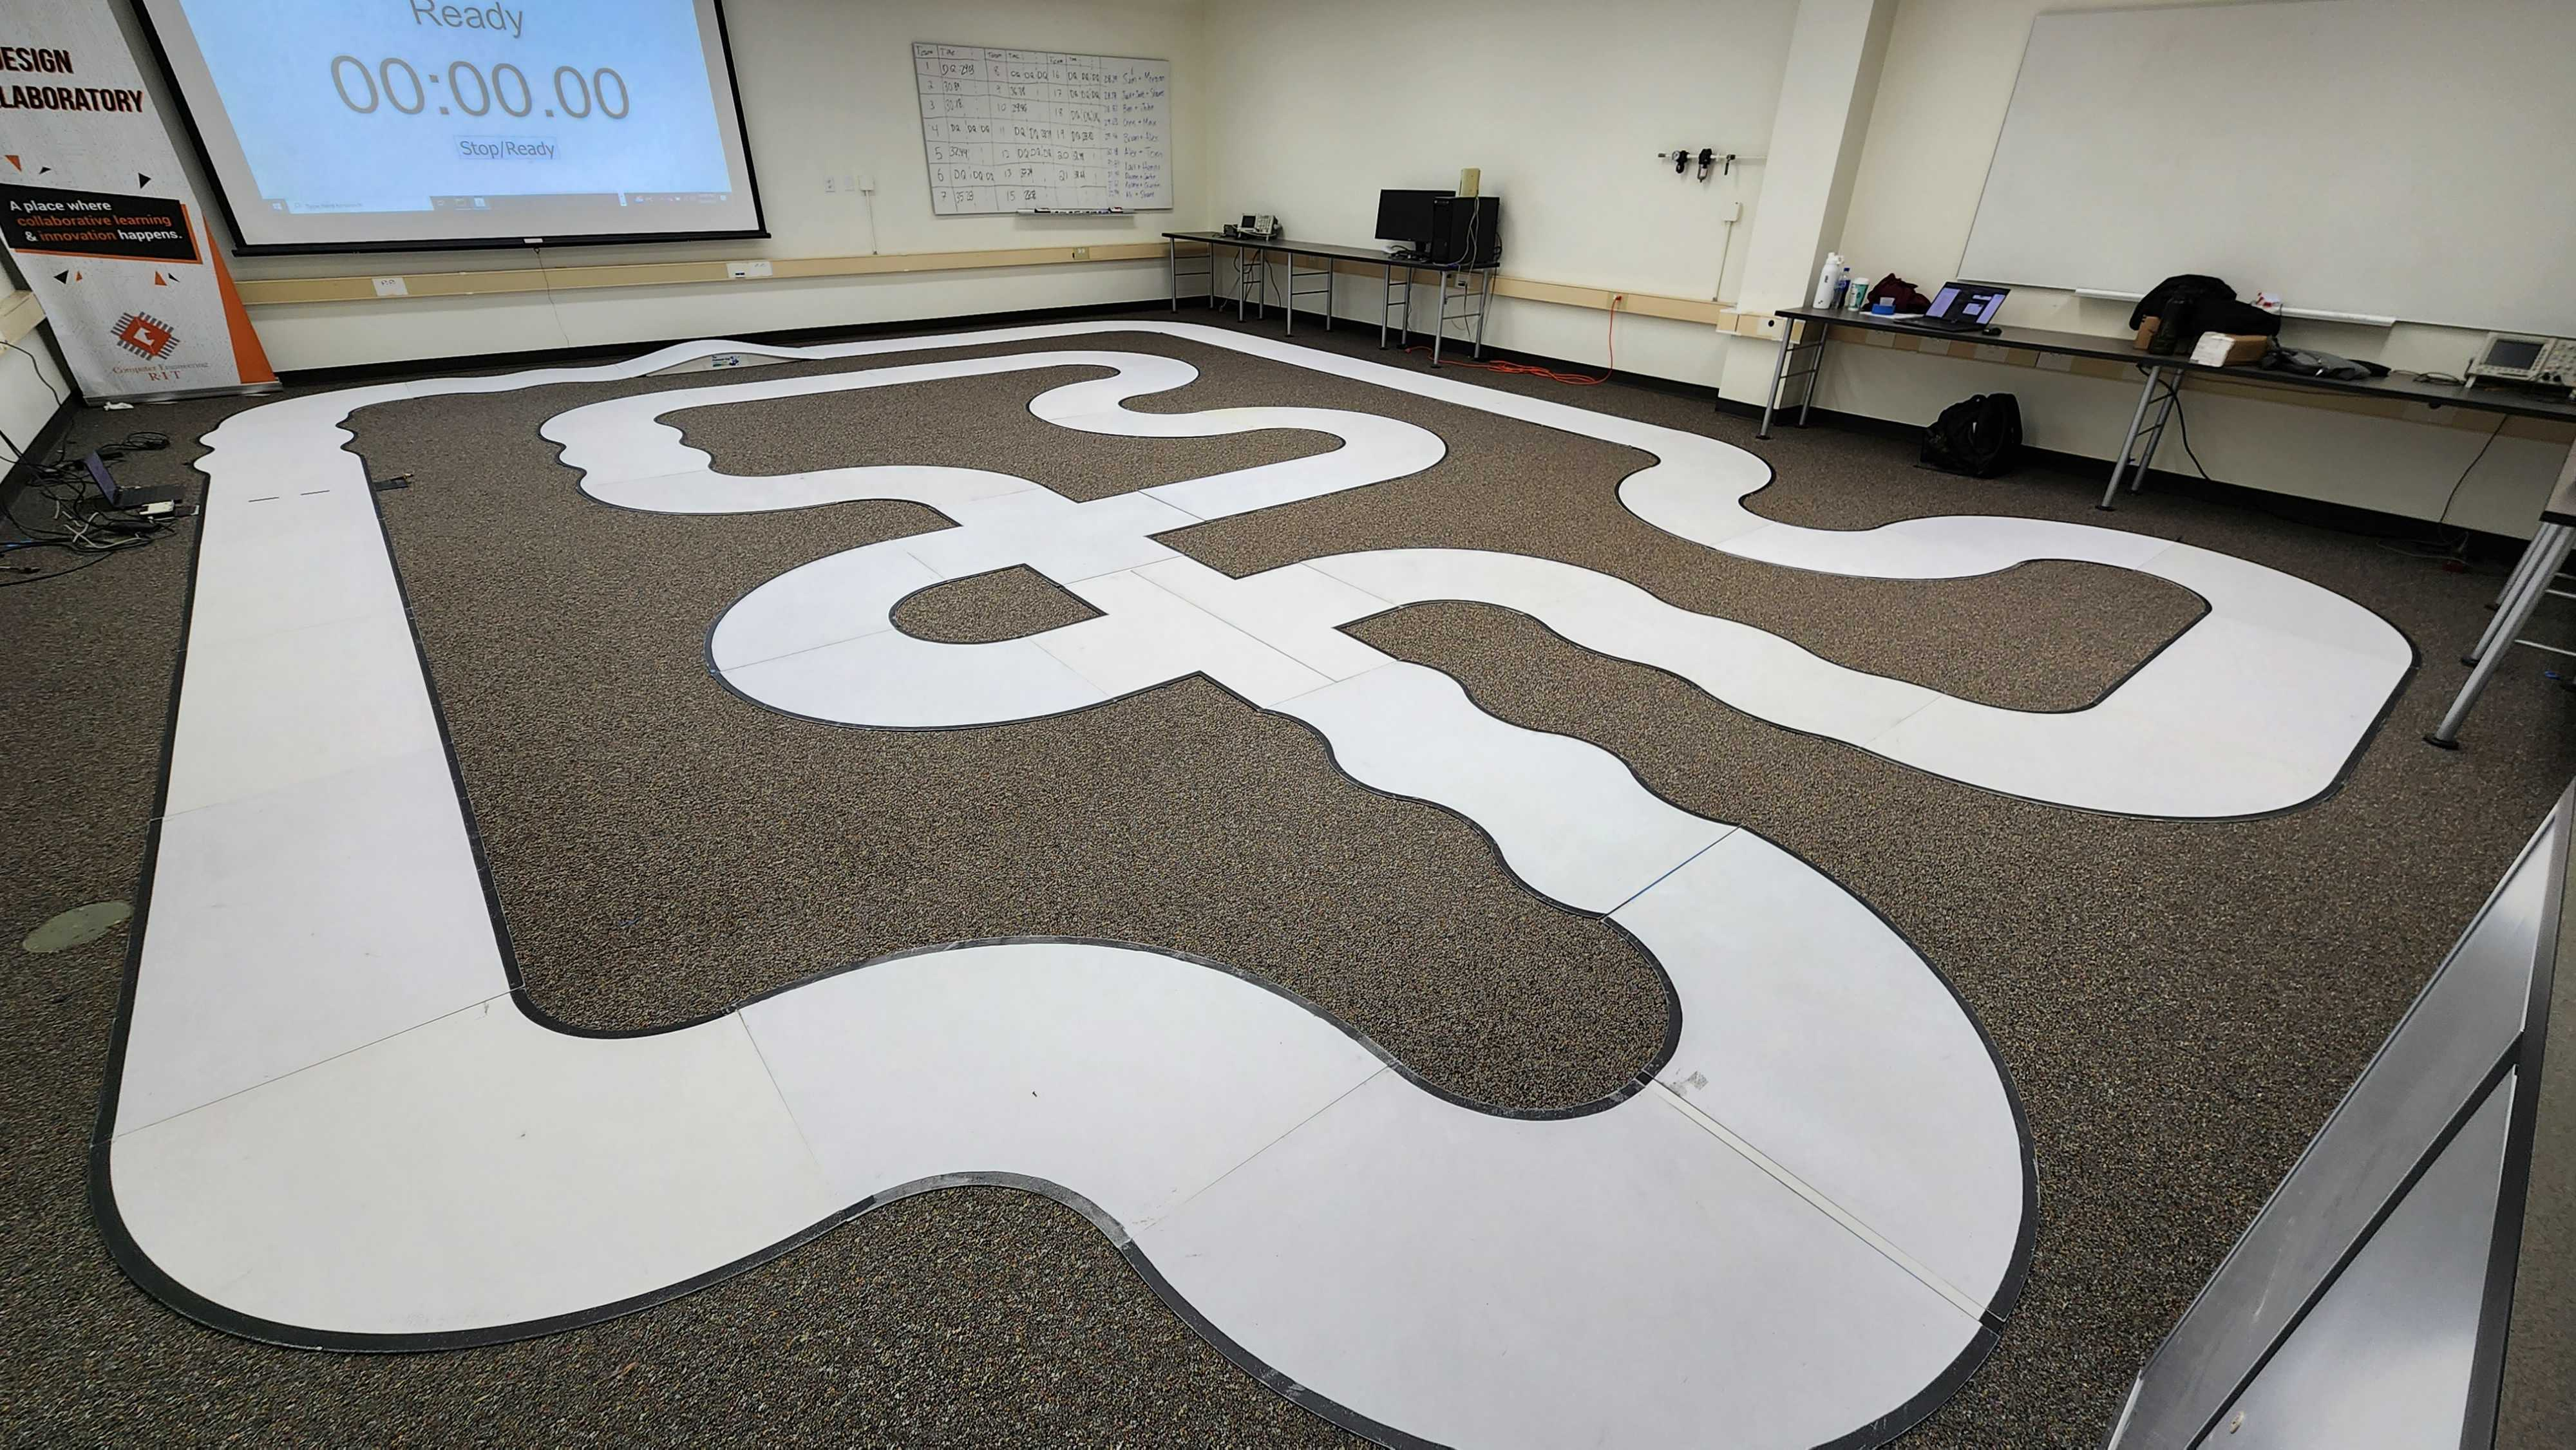
\includegraphics[width=0.45\textwidth]{images/track.jpg}}
	\caption{Racetrack for TI Cup.}
	\label{fig}
\end{figure}

\section{Background}

\subsection{Materials}

\begin{table}[htbp]
\caption{Bill of Materials}
\begin{center}
\begin{tabular}{|c|c|c|}
\hline
Part & Qty & Cost (USD) \\
\hline
Parallax TSL-1401 Line Scan Camera & 1 & \$80.00 \\
\hline
Servo Steering Arms & 1 & \$17.99 \\
\hline
Motor Driver - RB-WAV-77 & 1 & \$28.9 \\
\hline
Car Chassis Kit - ROB0170 & 1 & \$98.75 \\
\hline
Brushed DC Motor Kit - KIT0167 & 1 & \$25.00 \\
\hline
UCTRONICS Module 12864 SSD1306 OLED & 1 & \$6.99 \\
\hline
Bluetooth Module HM-10 & 1 & \$10.99 \\
\hline
Tenergy 7.2V High Capacity 6-Cell Battery Pack & 1 & \$39.99 \\
\hline
Sourcingpower Universal RC Battery Charger & 1 & \$19.99 \\
\hline
Fielect 5Pcs F-F 6Pin Jumper Wire Ribbon Cable & 1 & \$6.69 \\
\hline
5pcs Tamiya Male Power Connector Cable & 1 & \$8.68 \\
\hline
Zip Ties & 1 & \$18.99 \\
\hline
\textbf{Total} & & \textbf{\$363.05} \\
\hline
\end{tabular}
\label{billOfMaterials}
\end{center}
\end{table}

\begin{figure}[htbp]
	\centerline{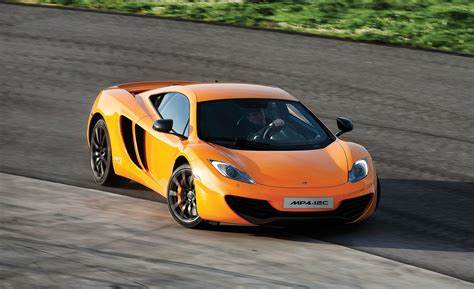
\includegraphics[width=0.45\textwidth]{images/car.jpg}}
	\caption{Car.}
	\label{fig}
\end{figure}

\subsection{PID theory}

\section{Proposed Method}

\section{Results}

\subsection{Race Results}


\section*{Acknowledgments}

\begin{thebibliography}{00}
\bibitem{b1} G. Eason, B. Noble, and I. N. Sneddon, ``On certain integrals of Lipschitz-Hankel type involving products of Bessel functions,'' Phil. Trans. Roy. Soc. London, vol. A247, pp. 529--551, April 1955.
\bibitem{b2} J. Clerk Maxwell, A Treatise on Electricity and Magnetism, 3rd ed., vol. 2. Oxford: Clarendon, 1892, pp.68--73.
\bibitem{b3} I. S. Jacobs and C. P. Bean, ``Fine particles, thin films and exchange anisotropy,'' in Magnetism, vol. III, G. T. Rado and H. Suhl, Eds. New York: Academic, 1963, pp. 271--350.
\bibitem{b4} K. Elissa, ``Title of paper if known,'' unpublished.
\bibitem{b5} R. Nicole, ``Title of paper with only first word capitalized,'' J. Name Stand. Abbrev., in press.
\bibitem{b6} Y. Yorozu, M. Hirano, K. Oka, and Y. Tagawa, ``Electron spectroscopy studies on magneto-optical media and plastic substrate interface,'' IEEE Transl. J. Magn. Japan, vol. 2, pp. 740--741, August 1987 [Digests 9th Annual Conf. Magnetics Japan, p. 301, 1982].
\bibitem{b7} M. Young, The Technical Writer's Handbook. Mill Valley, CA: University Science, 1989.
\end{thebibliography}

\end{document}
